% \documentclass[aspectratio=169,notes]{beamer}
\documentclass[aspectratio=169]{beamer}
\usetheme[faculty=phil]{fibeamer}
\usepackage{polyglossia}
\setmainlanguage{english} %% main locale instead of `english`, you
%% can typeset the presentation in either Czech or Slovak,
%% respectively.
\setotherlanguages{russian} %% The additional keys allow
%%
%%   \begin{otherlanguage}{czech}   ... \end{otherlanguage}
%%   \begin{otherlanguage}{slovak}  ... \end{otherlanguage}
%%
%% These macros specify information about the presentation
\title[MaM]{Mechanics and Machines, Lecture 7} %% that will be typeset on the
\subtitle{Links, Joints, Connections
\\ Shafts, Axles, Shafts couplings \\   
Bearings} %% title page.
\author{Oleg Bulichev}
%% These additional packages are used within the document:
\usepackage{ragged2e}  % `\justifying` text
\usepackage{booktabs}  % Tables
\usepackage{tabularx}
\usepackage{tikz}      % Diagrams
\usetikzlibrary{calc, shapes, backgrounds}
\usetikzlibrary{decorations.pathreplacing,calligraphy,calc,graphs}
\usepackage{amsmath, amssymb}
\usepackage{url}       % `\url`s
\usepackage{listings}  % Code listings
% \usepackage{subfigure}
\usepackage{floatrow}
\usepackage{subcaption}
\usepackage{mathtools}
\usepackage{todonotes}
\usepackage{fontspec}
\usepackage{multicol}
\usepackage{pdfpages}
\usepackage{wrapfig}
\usepackage{animate}
\usepackage{booktabs}
\usepackage{multirow}
% \usepackage{graphicx}
\usepackage{colortbl}

\graphicspath{{resources/}}
\frenchspacing

\setbeamertemplate{caption}[numbered]
\usetikzlibrary{graphs}

% \usepackage[backend=biber,style=ieee,autocite=footnote]{biblatex}
% \addbibresource{biblio.bib}
% \DefineBibliographyStrings{english}{%
%   bibliography = {References},}

\newcommand{\oleg}[2][] {\todo[color=red, #1] {OLEG:\\ #2}}
\newcommand{\fbckg}[1]{\usebackgroundtemplate{\includegraphics[width=\paperwidth]{#1}}}%frame background

\usepackage[framemethod=TikZ]{mdframed}
\newcommand{\dbox}[1]{
\begin{mdframed}[roundcorner=3pt, backgroundcolor=yellow, linewidth=0]
\vspace{1mm}
{#1}
\vspace{1mm}
\end{mdframed}
}

\begin{document}
\setlength{\abovedisplayskip}{0pt}
\setlength{\belowdisplayskip}{0pt}
\setlength{\abovedisplayshortskip}{0pt}
\setlength{\belowdisplayshortskip}{0pt}

\fbckg{fibeamer/figs/title_page.png}
\frame[c]{\setcounter{framenumber}{0}
    \usebeamerfont{title}%
    \usebeamercolor[fg]{title}%
    \begin{minipage}[b][6.5\baselineskip][b]{\textwidth}%
        \textcolor{black}{\raggedright\inserttitle}
    \end{minipage}
    % \vskip-1.5\baselineskip

    \usebeamerfont{subtitle}%
    \usebeamercolor[fg]{framesubtitle}%
    \begin{minipage}[b][3\baselineskip][b]{\textwidth}
        \raggedright%
        \insertsubtitle%
    \end{minipage}
    \vskip.25\baselineskip
}
%   \frame[c]{\maketitle}

\fbckg{fibeamer/figs/common.png}

\note{\scriptsize \begin{itemize}
        \item \ 
    \end{itemize}}

\begin{frame}[t]{Mechanism}
\framesubtitle{}
    \vspace{-0.6cm}
    \begin{figure}[H]
        \centering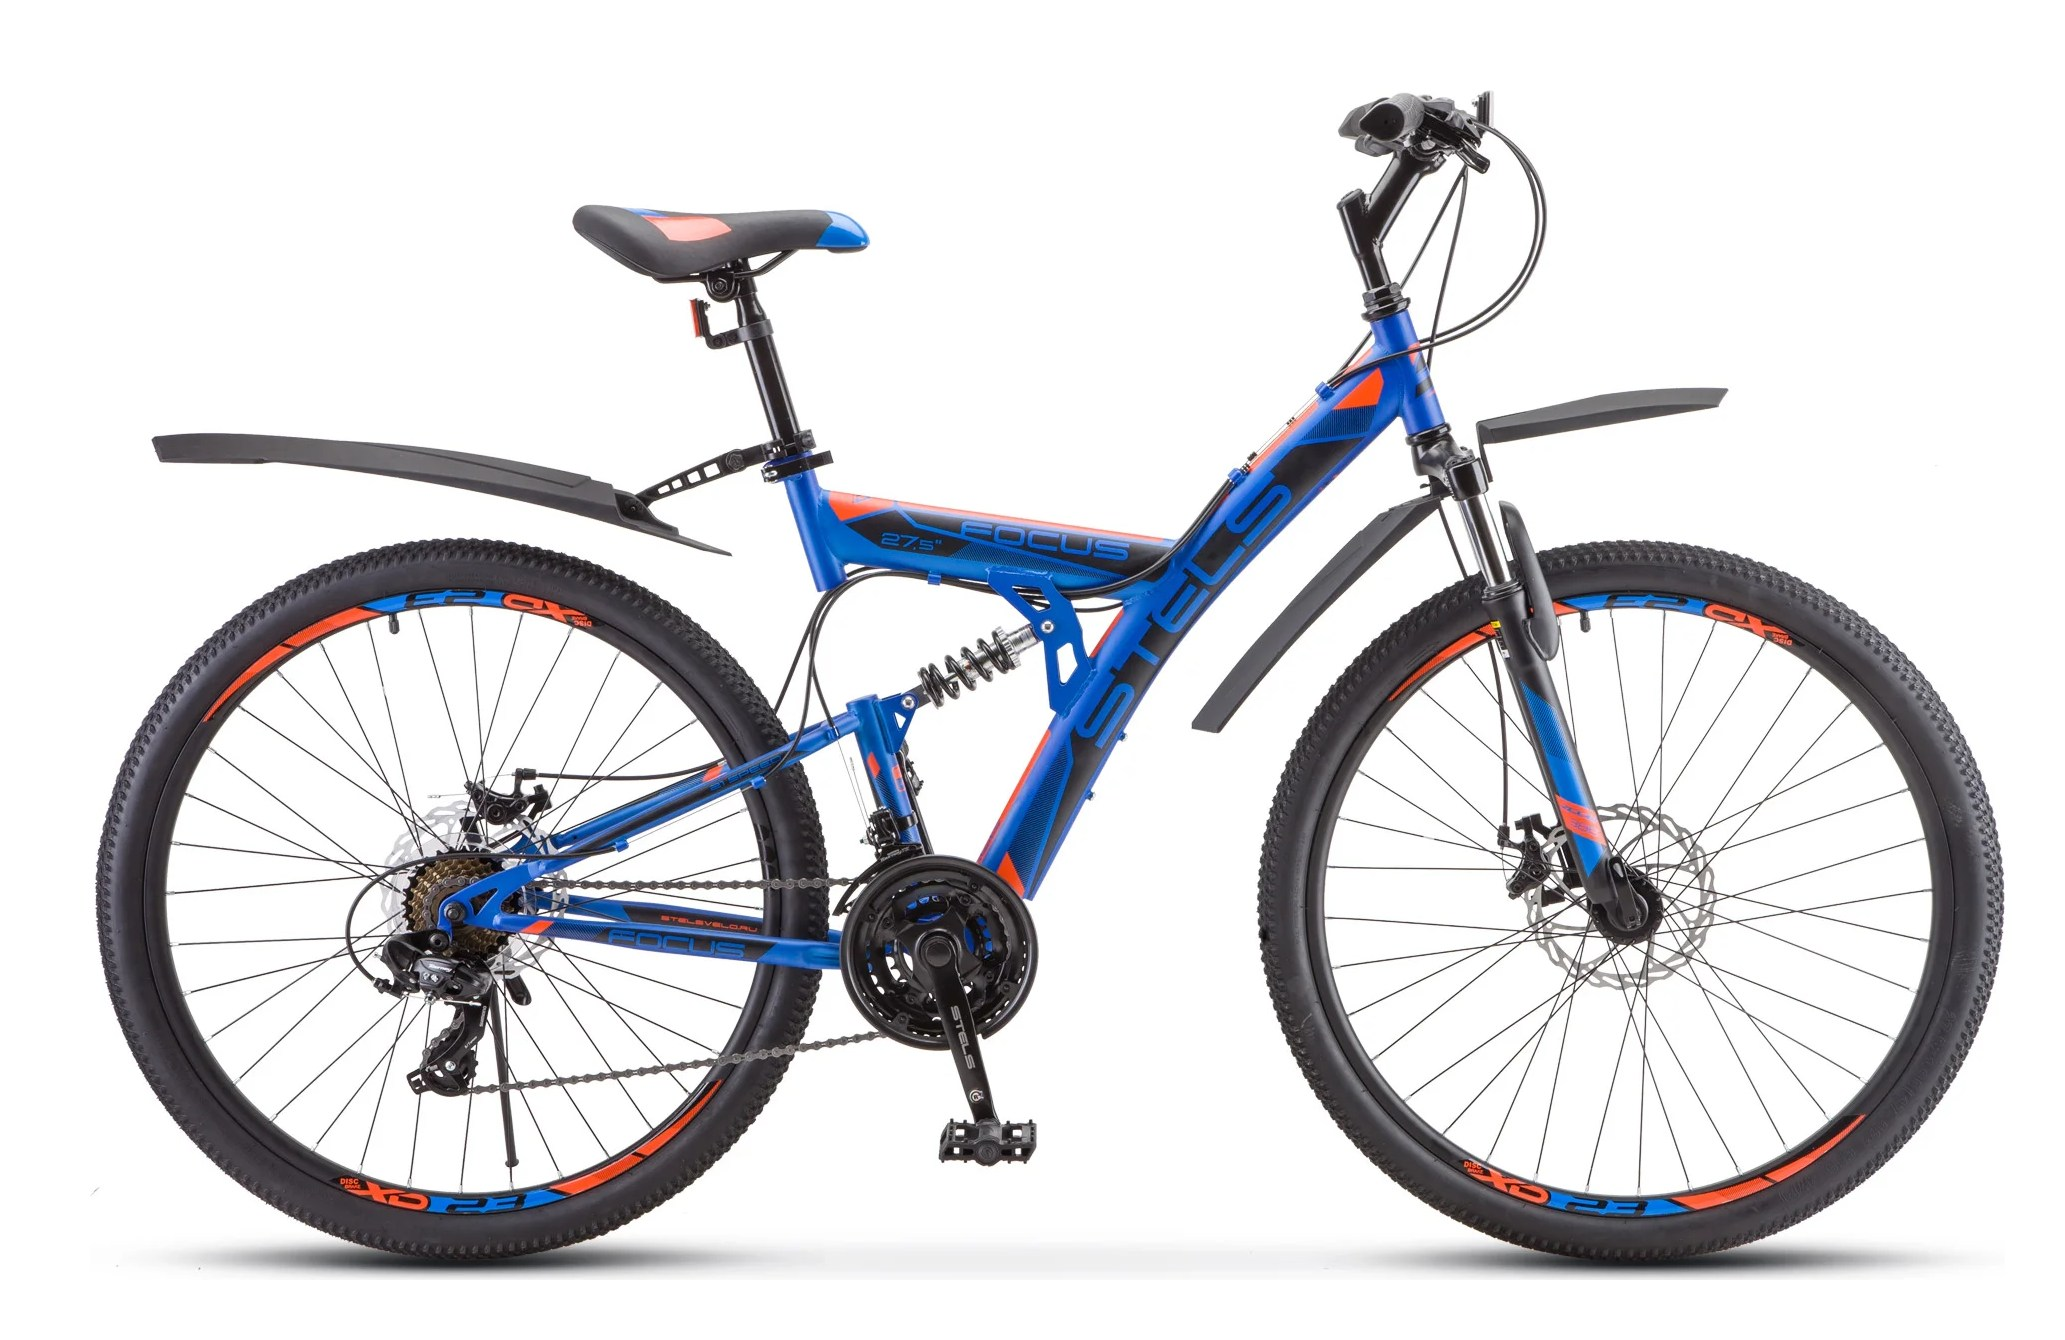
\includegraphics[height=6cm,width=1\textwidth,keepaspectratio]{bike.jpg}
        \label{fig:bike.jpg}
    \end{figure}
\end{frame}

\begin{frame}[t]{What does the mechanism consist of?}
\framesubtitle{}
    \begin{itemize}
        \item Links
        \item Joints
        \item Connections: permanent and detachable
    \end{itemize}
\end{frame}

\begin{frame}[t]{Links}
\framesubtitle{Types (my classification)}
\vspace{-0.7cm}
\begin{figure}[H]
    \begin{subfigure}{0.49\textwidth}
        \centering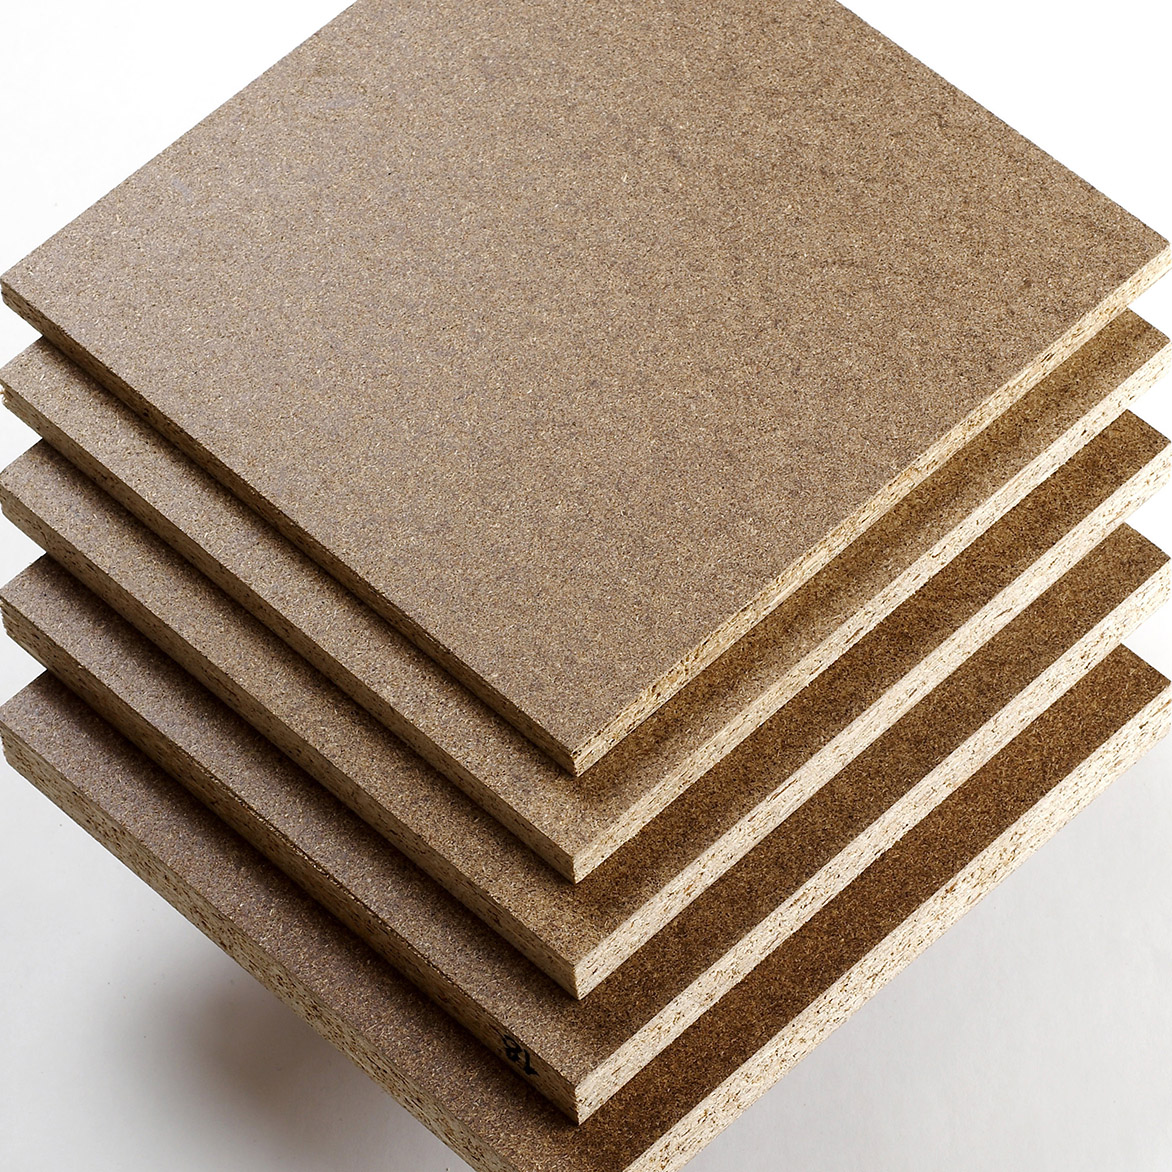
\includegraphics[height=2.4cm,width=1\textwidth,keepaspectratio]{sheet.jpg}
        \caption*{Sheet (Листовой материал): plywood (фанера)}
        \label{fig:sheet.jpg}
    \end{subfigure}
    \begin{subfigure}{0.49\textwidth}
        \centering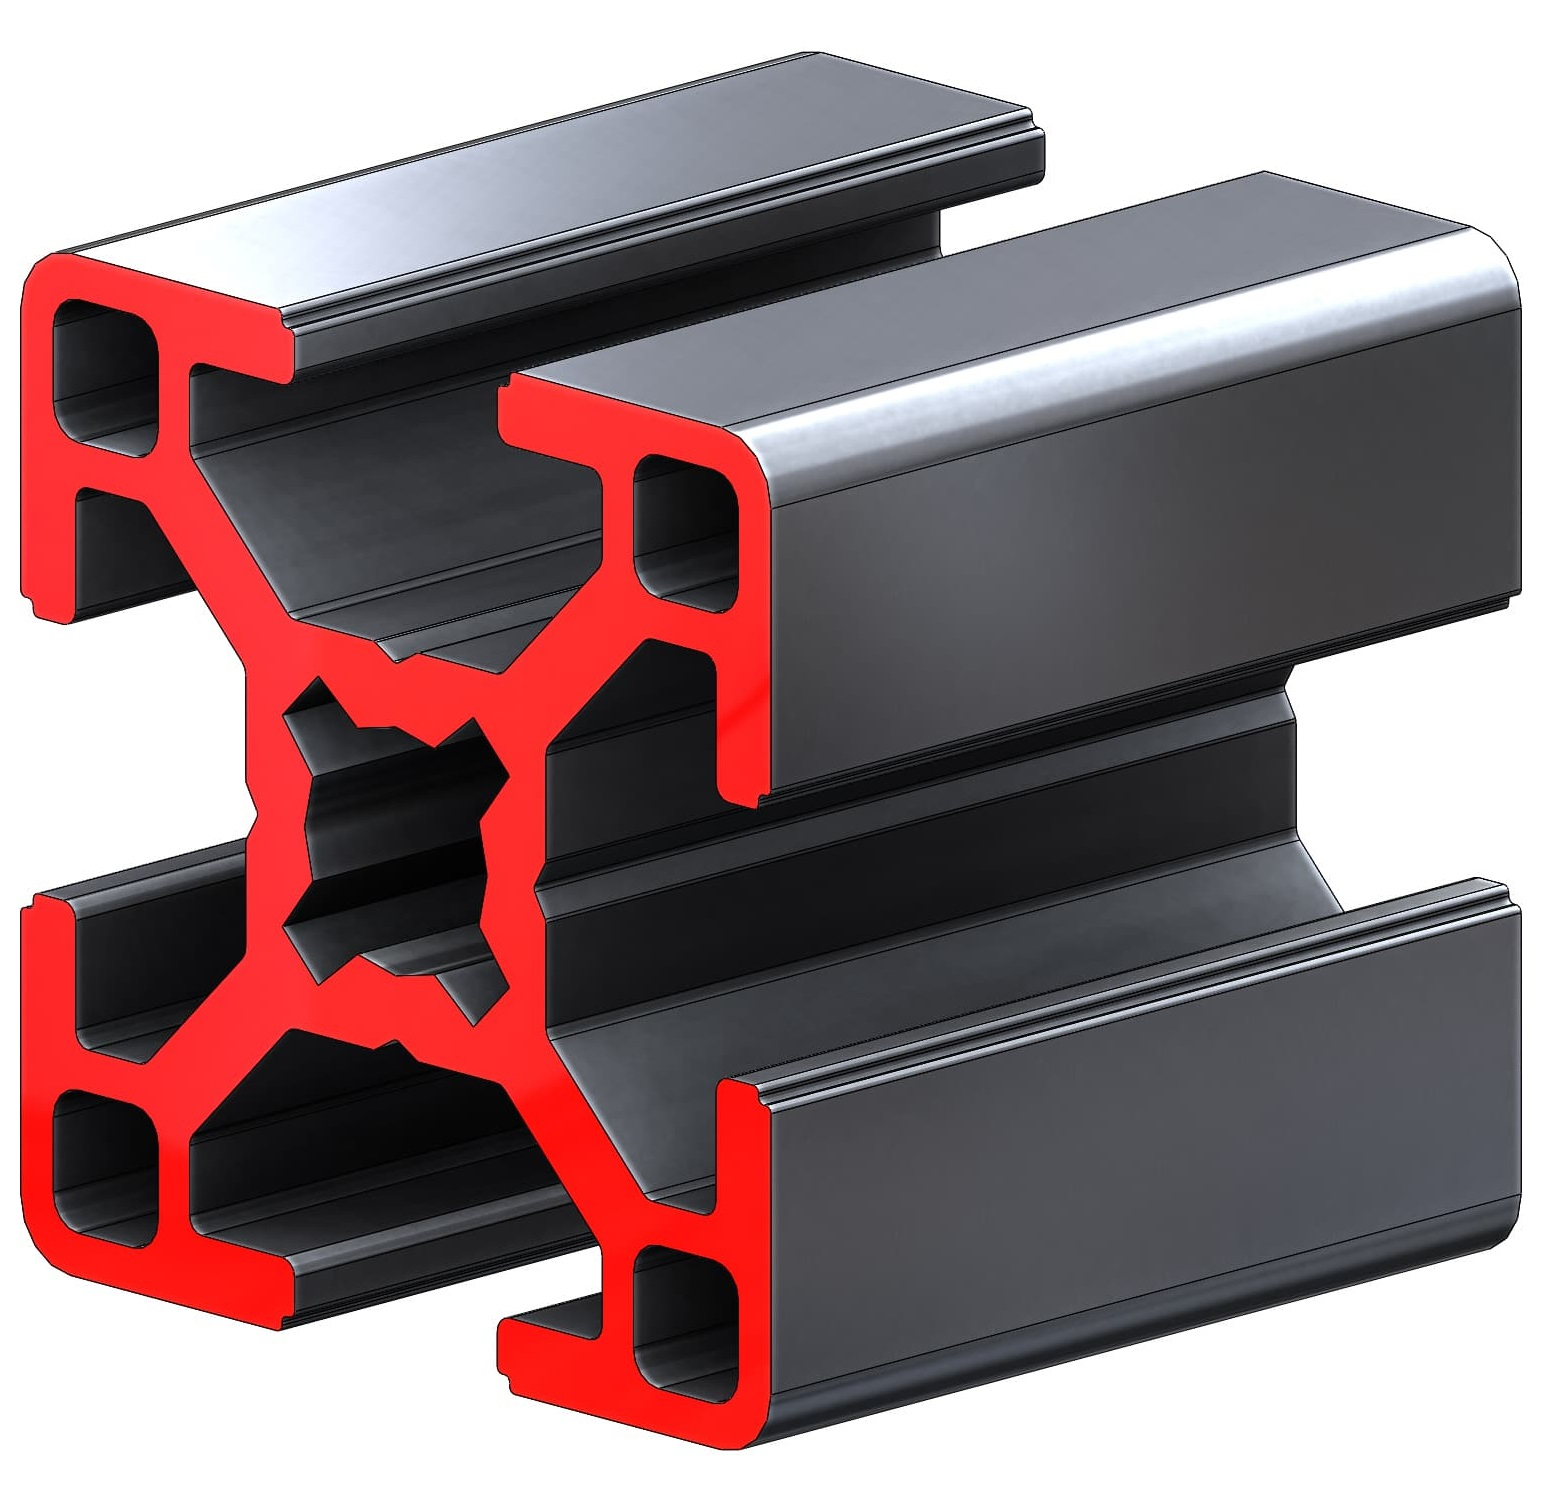
\includegraphics[height=2.4cm,width=1\textwidth,keepaspectratio]{tslot.jpg}
        \caption*{Profile (профиль): T-slot (Конструкционный профиль)}
        \label{fig:tslot.jpg}
    \end{subfigure}

    \begin{subfigure}{0.49\textwidth}
        \centering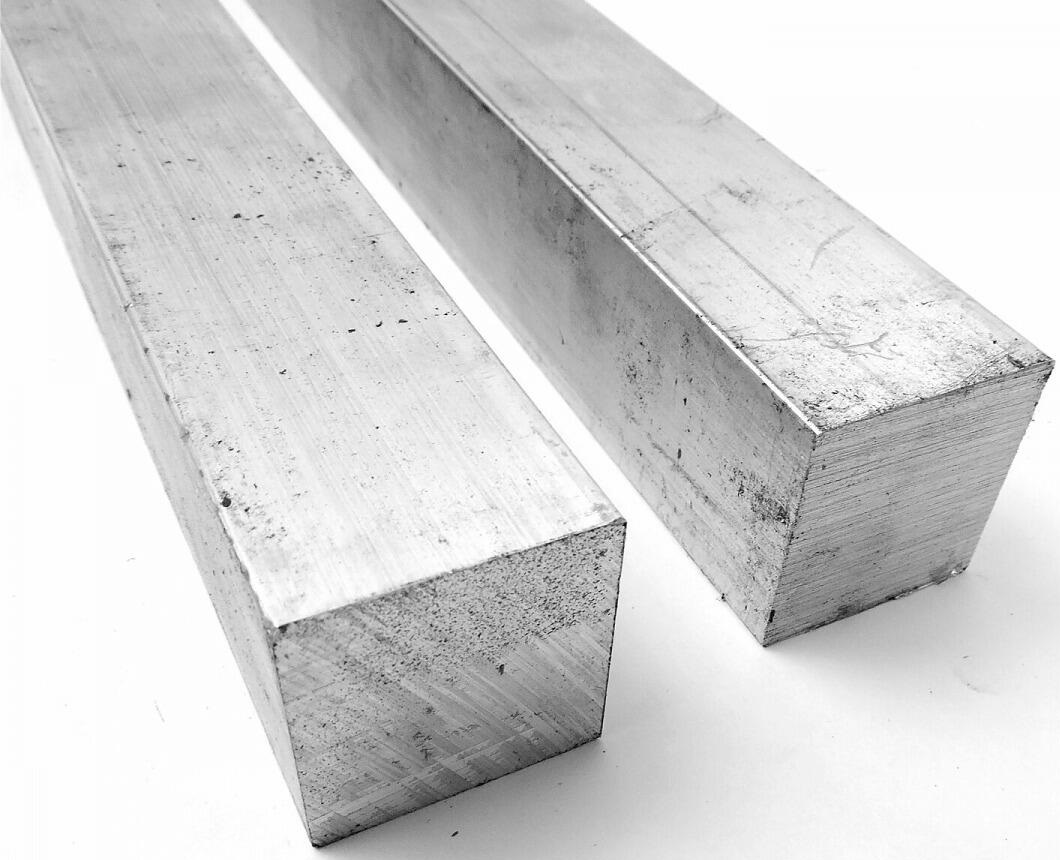
\includegraphics[height=2.4cm,width=1\textwidth,keepaspectratio]{beam.jpg}
        \caption*{Beam (Брус): al. bar (ал. брус)} 
        \label{fig:beam.jpg}
    \end{subfigure}
    \begin{subfigure}{0.49\textwidth}
        \centering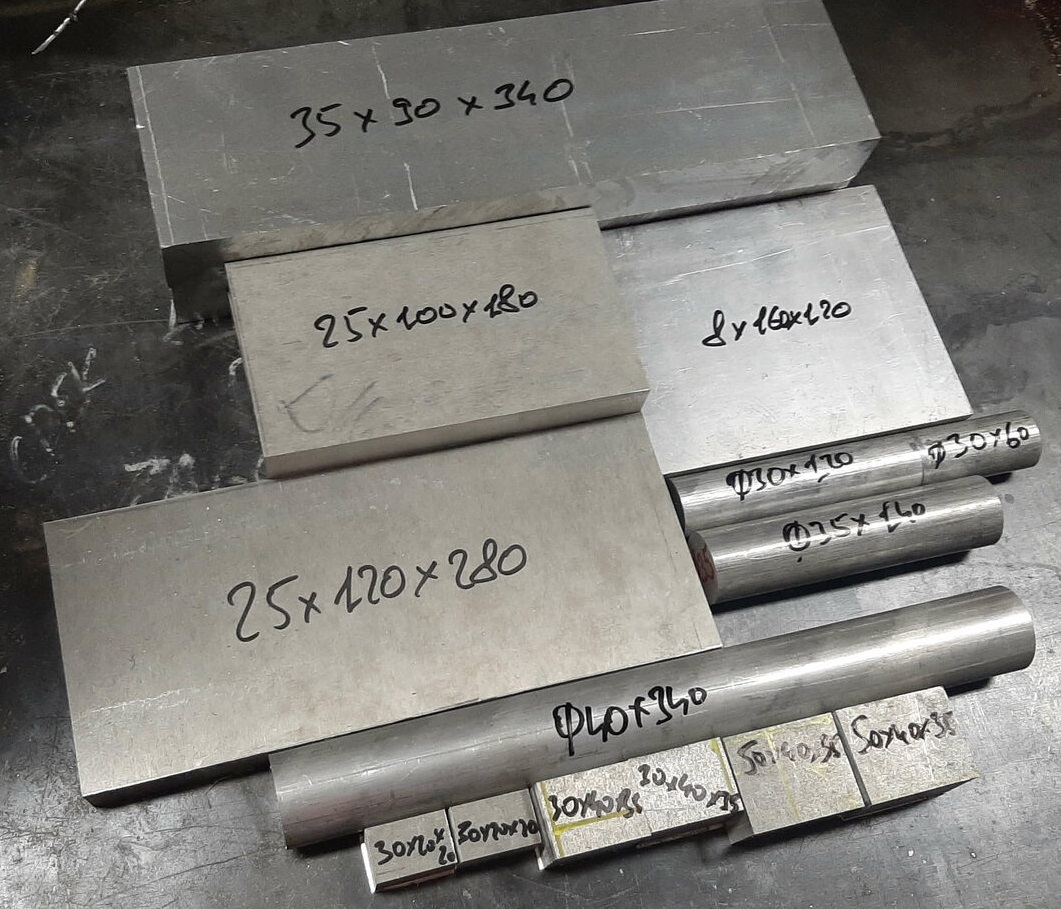
\includegraphics[height=2.4cm,width=1\textwidth,keepaspectratio]{cube.jpg}
        \caption*{Plate (плита): Aluminum billet (Заготовки)}
        \label{fig:file_name4}
    \end{subfigure}
\end{figure}
\end{frame}

\begin{frame}[c]{Joints}
\framesubtitle{}
    \centering \LARGE More info in \textbf{\href{https://github.com/Lupasic/MaM_Inno_2023/blob/main/lectures/3/MaM_lec3.pdf}{Lecture 3}}
\end{frame}

\begin{frame}[t]{Connections}
\framesubtitle{Classification}
    \vspace{-0.7cm}
    \begin{figure}[H]
        \begin{subfigure}{0.48\textwidth}
            \centering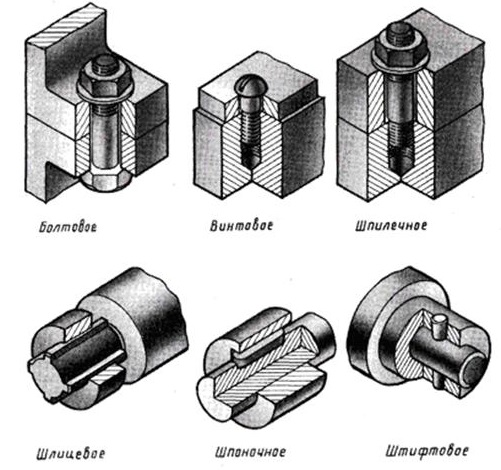
\includegraphics[height=5.5cm,width=1\textwidth,keepaspectratio]{detach.jpg}
            \caption*{Detachable (Разъемные)}
            \label{fig:detach.jpg}
        \end{subfigure}
        \begin{subfigure}{0.48\textwidth}
            \centering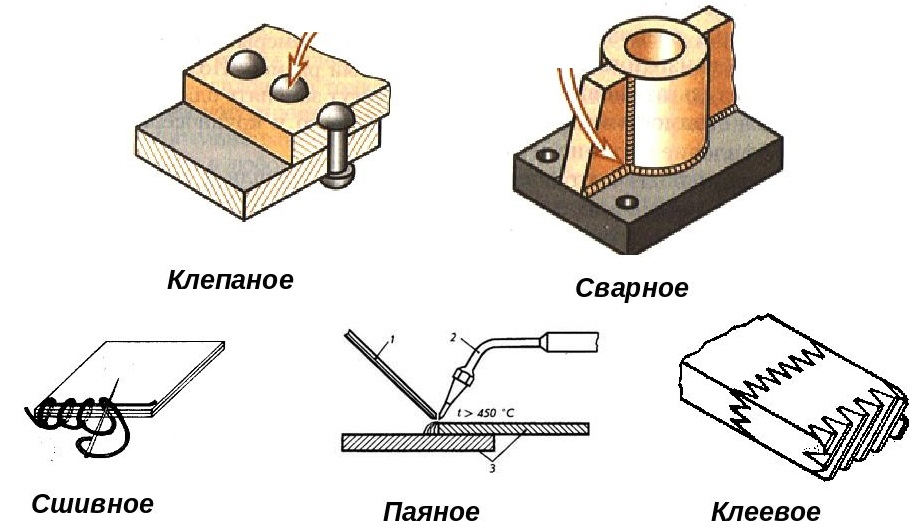
\includegraphics[height=5.5cm,width=1\textwidth,keepaspectratio]{fixed.jpg}
            \caption*{Permanent (Неразъемные)}
            \label{fig:fixed.jpg}
        \end{subfigure}
    \end{figure}
\end{frame}

\begin{frame}[t]{Shaft (Вал), Spindle (Шпиндель), Axle (Ось)}
    \framesubtitle{Video}
    \vspace{-0.6cm}
    \begin{figure}[H]
        \href{https://youtu.be/h04e2MpEHrM}{
            \centering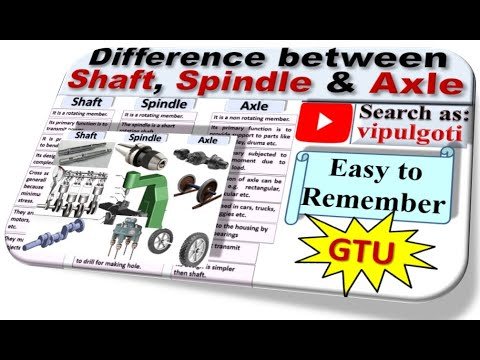
\includegraphics[height=6cm,width=1\textwidth,keepaspectratio]{shaft_spindel_axle_video.jpg}}
        % \caption{Click on a picture for a video}
        \label{fig:shaft_spindel_axle_video.jpg}
    \end{figure}
\end{frame}

\begin{frame}[t]{Shaft Coupling}
\framesubtitle{Intro}
    \begin{columns}[T,onlytextwidth]
        \begin{column}{0.49\textwidth}
            \textbf{The shaft coupling} is referred to as that mechanical component which is most commonly used for the purpose of \textit{connecting two rotating shaft}s like the driving shaft in order to let the driven shaft work for purpose of \textit{transmitting power}.
        \end{column}
        \begin{column}{0.49\textwidth}
            \begin{figure}[H]
                \centering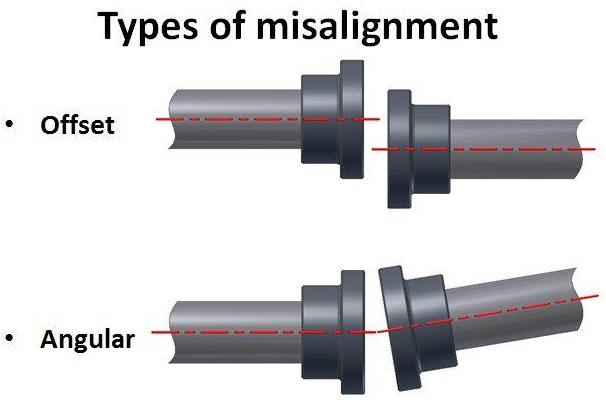
\includegraphics[height=4cm,width=1\textwidth,keepaspectratio]{misal_shafts.jpg}
                % \caption{caption_name}
                \label{fig:misal_shafts.jpg}
            \end{figure}
        \end{column}
    \end{columns}
\end{frame}

\begin{frame}[t]{Shaft Coupling}
    \framesubtitle{Video}
    \vspace{-0.6cm}
    \begin{figure}[H]
        \href{https://youtu.be/SPnTA3H2G7g}{
            \centering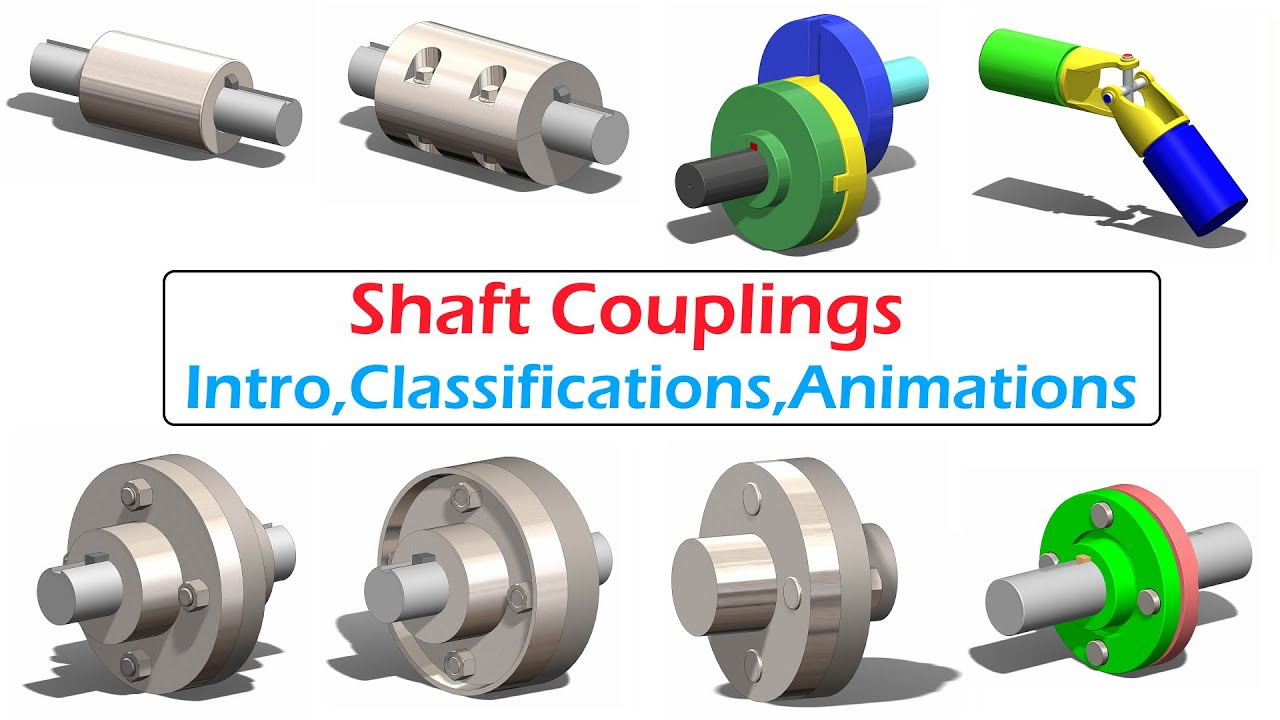
\includegraphics[height=6cm,width=1\textwidth,keepaspectratio]{shaft_coupling_video.jpg}}
        % \caption{Click on a picture for a video}
        \label{fig:shaft_coupling_video.jpg}
    \end{figure}
\end{frame}

\begin{frame}[t]{Types of shaft couplings}
\framesubtitle{}
    \vspace{-0.6cm}
    \begin{figure}[H]
        \centering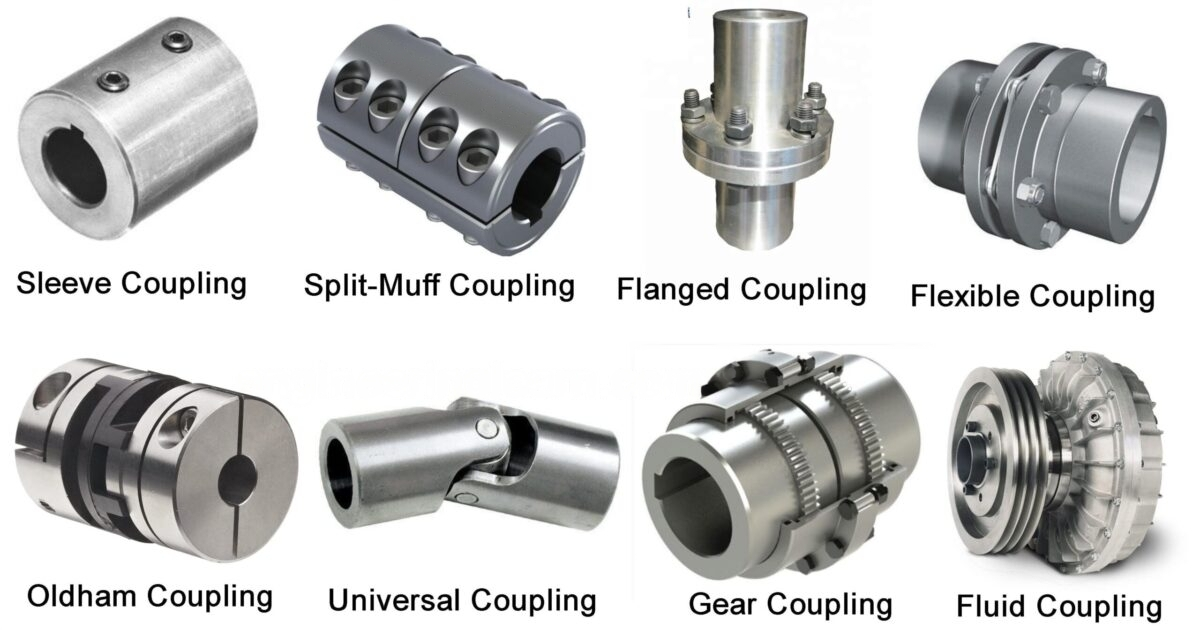
\includegraphics[height=6cm,width=1\textwidth,keepaspectratio]{couplings.jpeg}
        \label{fig:couplings.jpeg}
    \end{figure}
\end{frame}

\begin{frame}[t]{Practical usage of Shaft Couplings}
    \framesubtitle{Video}
    \vspace{-0.6cm}
    \begin{figure}[H]
        \href{https://youtu.be/q1bkBPtqEZw?t=178}{
            \centering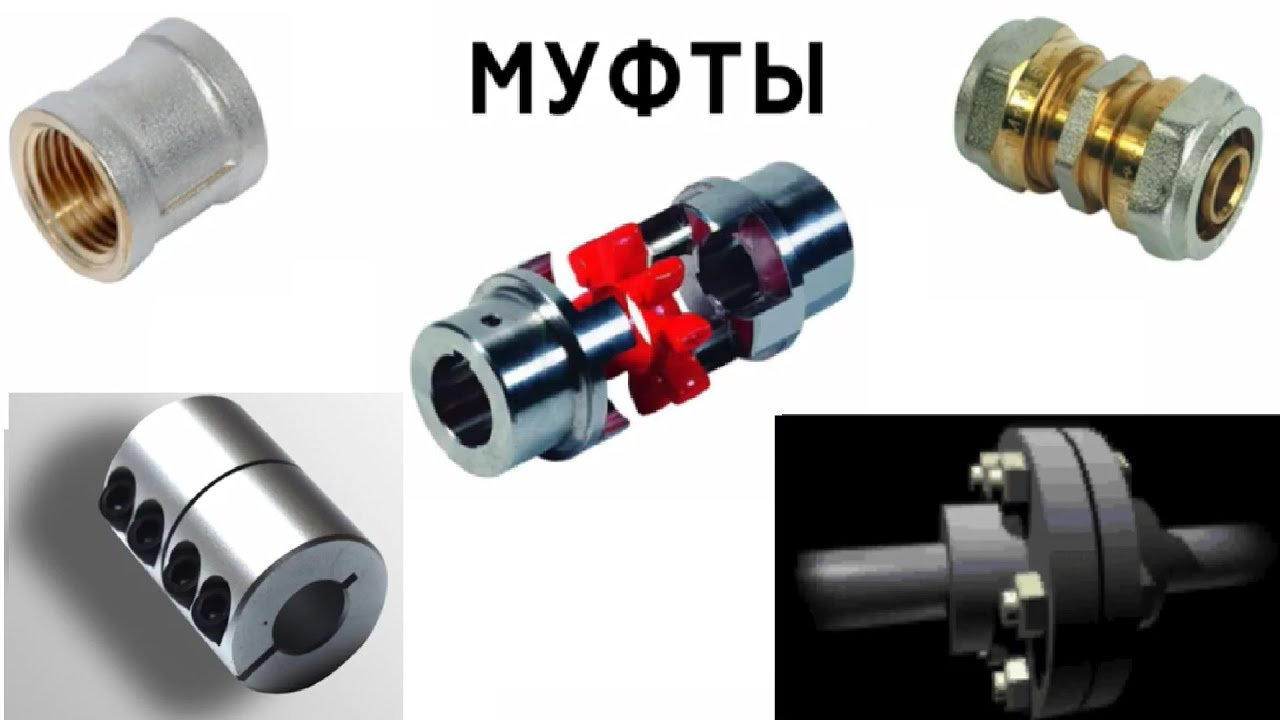
\includegraphics[height=6cm,width=1\textwidth,keepaspectratio]{muft_video.jpg}}
        \label{fig:muft_video.jpg}
    \end{figure}
\end{frame}

\begin{frame}[t]{Shafts + Shaft Couplings}
\framesubtitle{Reference material}
    \begin{itemize}
        \item \href{https://youtu.be/hm3V2G5VfWk}{Shafts (video, rus)}
        \item \href{https://youtu.be/PBasimGAhJw}{Classification of couplings, Types of couplings, Coupling types (Indian, video)}
        \item \href{https://engineeringlearn.com/shaft-coupling-definition-types-uses-working-principle-advantages-complete-guide/}{Text material about shaft couplings}
    \end{itemize}
\end{frame}

\begin{frame}[t]{Bearings}
\framesubtitle{Definition}
\vspace{-0.5cm}
    \begin{columns}[T,onlytextwidth]
        \begin{column}{0.39\textwidth}
            \textbf{Bearing} is a machine element that \textit{constrains relative motions} and is used to \textit{reduce the friction} between moving parts.
        \end{column}
        \begin{column}{0.59\textwidth}
            \begin{figure}[H]
                \centering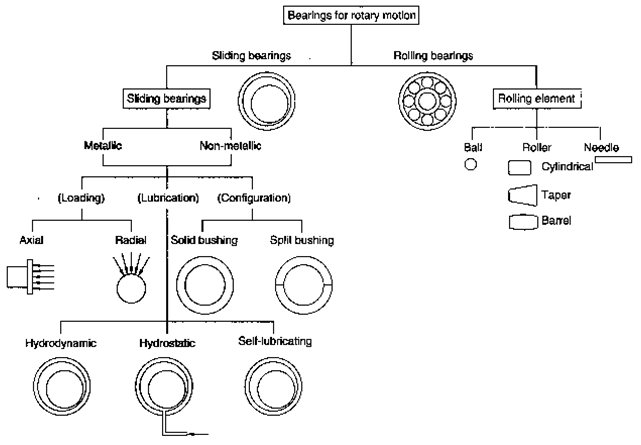
\includegraphics[height=5.5cm,width=1\textwidth,keepaspectratio]{bearing_conf.png}
                % \caption{caption_name}
                \label{fig:bearing_conf.png}
            \end{figure}
        \end{column}
    \end{columns}
\end{frame}

\

\begin{frame}[t]{Bearings}
    \framesubtitle{Reference material}
        \begin{itemize}
            \item \href{https://youtu.be/8q25EUszBSI}{Bearings 1}
            \item \href{https://youtu.be/QhTI8CnRic8}{Bearings 2}
            \item \href{https://youtu.be/Ezooa2dIyRA}{Linear Guideway}
            \item \href{https://youtu.be/leTXJqZeqPA}{Linear Ball bearings}
            \item \href{https://youtu.be/mXNd-2lTIpk}{uninstall and install bearings}
            \item \href{https://youtu.be/UAVXJHjPqKk}{Выбор посадки подшипников}
            \item \href{https://www.s-graciya.ru/upload/file/FAG/7-pr_pod_opor.pdf}{Проектирование подшипниковых опор}
            \item \href{https://youtu.be/3vaT1CAhKeQ}{Как раз про проектирование подшипниковых опор}
            \item \href{https://youtu.be/QCDovyEb7JM}{pillow block}
            \item \href{https://youtu.be/xTqEc2vfIEY}{Подшипники качения на руссокм}
            \item \href{https://youtu.be/Ptm3c5byXAY}{Подшипнии скольжения на русском}
        \end{itemize}
    \end{frame}

\begin{frame}[t]{Reference material}
    \framesubtitle{}
    \begin{enumerate}
        \item \href{https://www.youtube.com/watch?v=e4bWFgQTlxc}{List of Basic Mechanical Parts (video)}
        \item Mott R. L., Vavrek E. M., Wang J. Machine Elements in Mechanical Design, Ed. --- 2011
        \item Avallone E. A., Baumeister III T., Sadegh A. Marks' standard handbook for mechanical engineers. --- McGraw-Hill Education, 2007.
        \item Budynas R. G. et al. Shigley's mechanical engineering design. --- New York : McGraw-Hill, 2011.
        \item \href{https://engineeringbookspdf.com/category/mechanical-engineering-pdf-books/}{A lot of engineering books in english}
    \end{enumerate}

    % 
\end{frame}



\fbckg{fibeamer/figs/last_page.png}
\frame[plain]{}

\end{document}